\documentclass[sigconf, review=false, anonymous=false, authorversion=false, timestamp=false, authordraft=false]{acmart}

\usepackage{booktabs} % For formal tables
\usepackage{makecell} % Line break in cell
\usepackage{graphicx}
\usepackage{subcaption}
\usepackage{flushend}
\usepackage{listings}
\usepackage{xcolor}

% listings code formatting configuration
\colorlet{punct}{red!60!black}
\definecolor{background}{HTML}{EEEEEE}
\definecolor{delim}{RGB}{20,105,176}
\colorlet{numb}{magenta!60!black}

\lstdefinestyle{CodeStyle}{
    captionpos=b,
    basicstyle=\footnotesize\ttfamily,
    numbers=left,
    numberstyle=\scriptsize,
    stepnumber=1,
    numbersep=8pt,
    showstringspaces=false,
    breaklines=true,
    frame=lines,
    backgroundcolor=\color{background}
}

\lstdefinelanguage{JavaScript}{
    morekeywords={typeof, new, true, false, catch, function, return, null, catch, switch, var, if, in, while, do, else, case, break},
    morecomment=[s]{/*}{*/},
    morecomment=[l]//,
    morestring=[b]",
    morestring=[b]',
    style=CodeStyle
}

\lstdefinelanguage{json}{
    literate=
     *{0}{{{\color{numb}0}}}{1}
      {1}{{{\color{numb}1}}}{1}
      {2}{{{\color{numb}2}}}{1}
      {3}{{{\color{numb}3}}}{1}
      {4}{{{\color{numb}4}}}{1}
      {5}{{{\color{numb}5}}}{1}
      {6}{{{\color{numb}6}}}{1}
      {7}{{{\color{numb}7}}}{1}
      {8}{{{\color{numb}8}}}{1}
      {9}{{{\color{numb}9}}}{1}
      {:}{{{\color{punct}{:}}}}{1}
      {,}{{{\color{punct}{,}}}}{1}
      {\{}{{{\color{delim}{\{}}}}{1}
      {\}}{{{\color{delim}{\}}}}}{1}
      {[}{{{\color{delim}{[}}}}{1}
      {]}{{{\color{delim}{]}}}}{1},
    style=CodeStyle
}

\lstset{
    language=haskell,
    style=CodeStyle
}

% DOI and ISBN
\acmDOI{10.1145/3240508.3243656}
\acmISBN{978-1-4503-5665-7/18/10} % chktex 8

% Conference
\acmYear{2018}
\acmConference[MM '18]{2018 ACM Multimedia Conference}{October 22--26, 2018}{Seoul, Republic of Korea}
\acmBooktitle{2018 ACM Multimedia Conference (MM '18), October 22--26, 2018, Seoul, Republic of Korea}
\acmPrice{15.00}

% Copyright
\setcopyright{acmlicensed}
\copyrightyear{2018}

% "ACM Reference format" and CCS
\settopmatter{printacmref=true, printccs=true, printfolios=false, authorsperrow=4}

% Remove headers for camera ready submission
\fancyhead{}


\begin{document}
\title{Web-Based Configurable Image Annotations}


\author{Matthieu Pizenberg}
% \authornote{}
\orcid{0000-0001-6241-6325} % chktex 8
\affiliation{%
  \institution{University of Toulouse}
%   \streetaddress{41 Allées Jules Guesde}
%   \city{Toulouse}
%   \country{France}
%   \postcode{31013}
}
\email{matthieu@pizenberg.fr}

\author{Axel Carlier}
\orcid{0000-0002-6838-3445} % chktex 8
\affiliation{%
  \institution{University of Toulouse}
%   \streetaddress{41 Allées Jules Guesde}
%   \city{Toulouse}
%   \country{France}
%   \postcode{31013}
}
\email{axel.carlier@irit.fr}

\author{Emmanuel Faure}
\orcid{0000-0003-2787-0885} % chktex 8
\affiliation{%
  \institution{CNRS\ -\ IRIT}
%   \streetaddress{2 rue Camichel}
%   \city{Toulouse}
%   \country{France}
%   \postcode{31071}
}
\email{emmanuel.faure@irit.fr}

\author{Vincent Charvillat}
\affiliation{%
  \institution{University of Toulouse}
%   \streetaddress{41 Allées Jules Guesde}
%   \city{Toulouse}
%   \country{France}
%   \postcode{31013}
}
\email{vincent.charvillat@irit.fr}

% The default list of authors is too long for headers
\renewcommand{\shortauthors}{M. Pizenberg et al.}

% Add the sentence required for OSS competition submission
\makeatletter
\def\@teaserfigures{\vskip 2mm
\centerline{SUBMITTED to ACM MULTIMEDIA 2018 OPEN SOURCE SOFTWARE COMPETITION}
\vskip 2mm}
\makeatother

% Teaser figure
\begin{teaserfigure}
  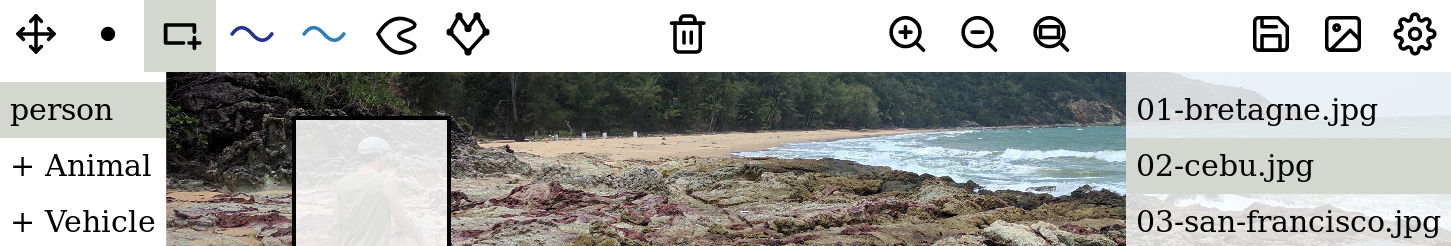
\includegraphics[width=\textwidth]{img/annotation-app-thin.jpg}
  \caption{Screenshot of the interface of our image annotation Web application.}%
  \label{fig:teaser}
\end{teaserfigure}

% Abstract
\begin{abstract}
We introduce a new application for annotating images, with the purpose
of constituting training datasets for machine learning algorithms.
Our open-source software is meant to be easily used and deployed,
configured to meet the annotation needs of any use case, and
embeddable in crowdsourcing campaigns using the Amazon Mechanical
Turk service.
\end{abstract}

% The code below should be generated by the tool at
% http://dl.acm.org/ccs.cfm
\begin{CCSXML}
<ccs2012>
<concept>
    <concept_id>10010405.10010497.10010510.10010513</concept_id>
    <concept_desc>Applied computing~Annotation</concept_desc>
    <concept_significance>500</concept_significance>
</concept>
</ccs2012>
\end{CCSXML}

\ccsdesc[500]{Applied computing~Annotation}

\keywords{annotation; open source software; dataset}

\maketitle

\section{Introduction}

Image annotations are required in a wide range of applications
including image classification (which requires textual labels),
object detection (bounding boxes), or image segmentation (pixel-wise classification).
The rise and successes of deep learning lead to an increasing need for annotations,
as training sets should be of a large size for these algorithms to be efficient.
Yet, in many cases, researchers spend time and resources
to create ad hoc tools to prepare those datasets.
The application we present in this paper aims at providing a customizable tool
to fulfill most image annotation needs.

\begin{table*}[ht]

\begin{tabular}{lclllcc}
Application
	& Year
    & Tools
    & \makecell[l]{Configurable\\interface}
    & \makecell[l]{Tasks\\management}
    & Type
    & License \\
    \midrule
LabelMe
	& 2008
    & bbox, polygon, iterative semi-automatic segmentation
    & no
    & Mturk integration
    & server
    & OSS \\
VIA
	& 2016
    & bbox, polygon, point, circle, ellipse
    & no
    & no
    & client
    & OSS \\
Labelbox
	& 2018
    & bbox, polygon, point, line
    & yes
    & yes
    & server
    & private \\
Dataturks
	& 2018
    & bbox, polygon
    & no
    & yes
    & server
    & private \\
Ours
	& 2018
    & bbox, polygon, point, stroke, outline
    & yes
    & Mturk integration
    & client
    & OSS \\
\end{tabular}

\caption{Most relevant image annotation Web applications.}%
\label{tab:web-apps}
\end{table*}

% \begin{figure*}[ht]
%     \centering
%     \begin{subfigure}[b]{0.575\textwidth}
%         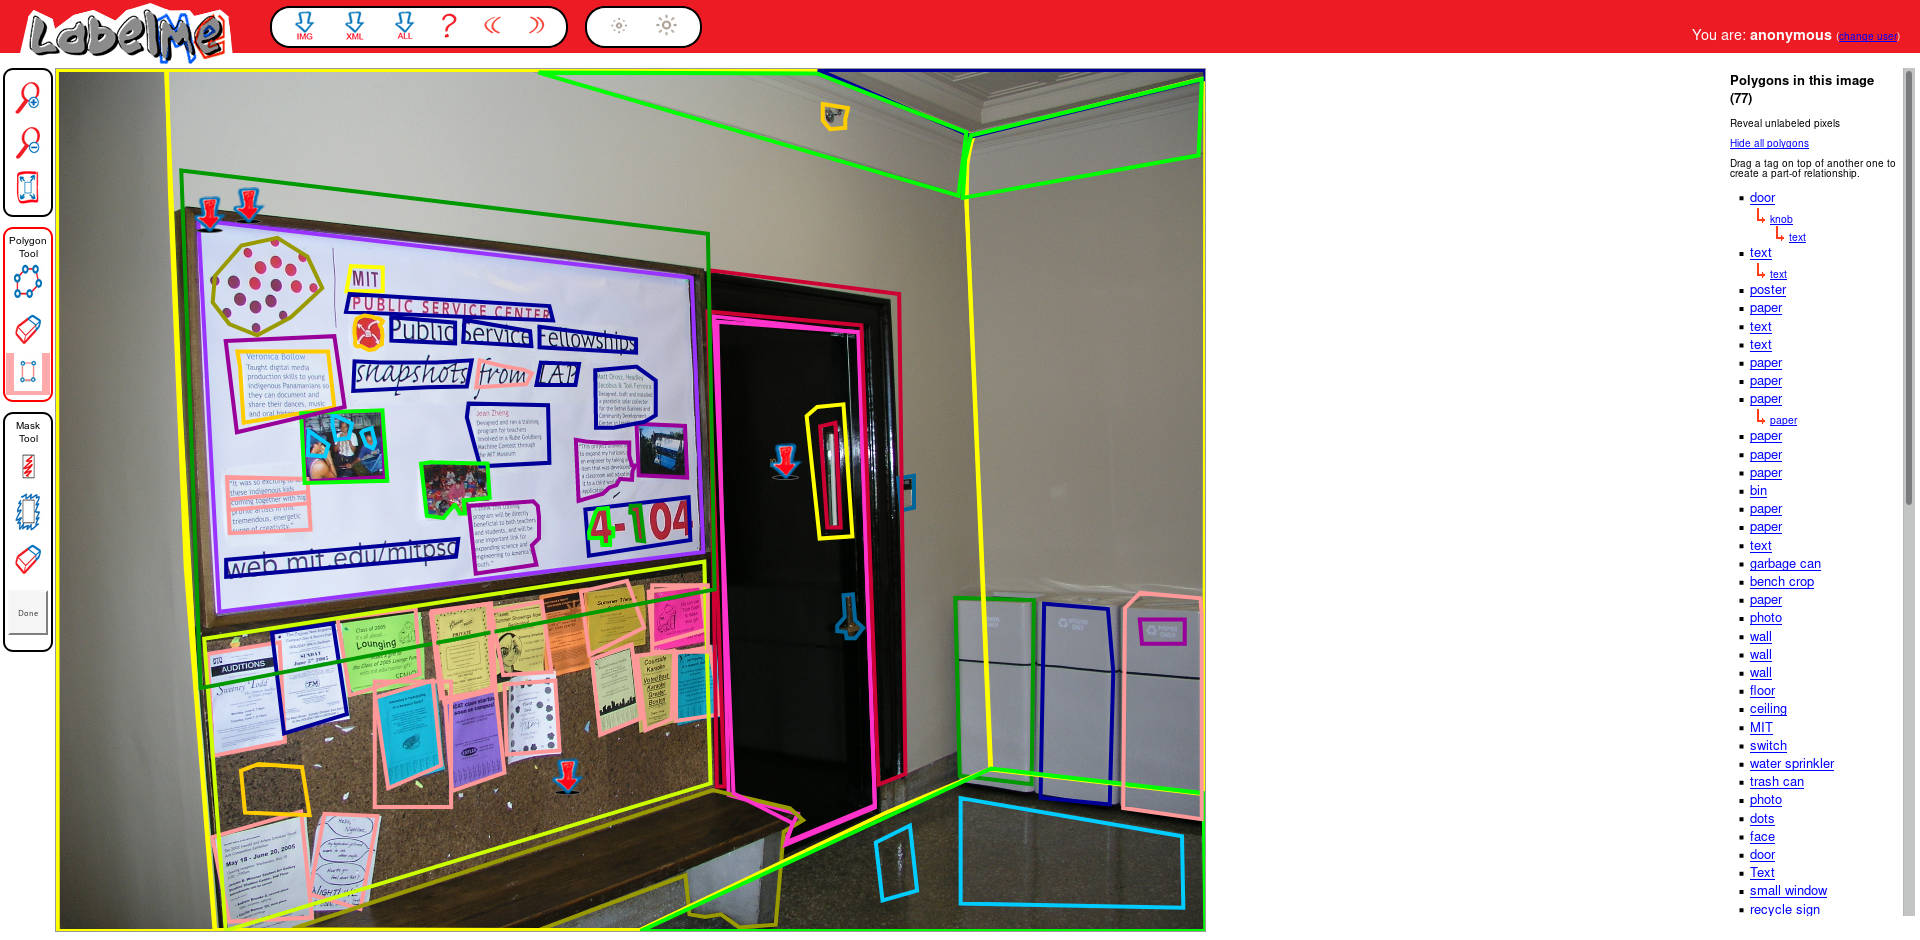
\includegraphics[width=\textwidth]{img/labelme.jpg}
%         \caption{Labelme}
%     \end{subfigure}
%     \hfill
%     \begin{subfigure}[b]{0.405\textwidth}
%         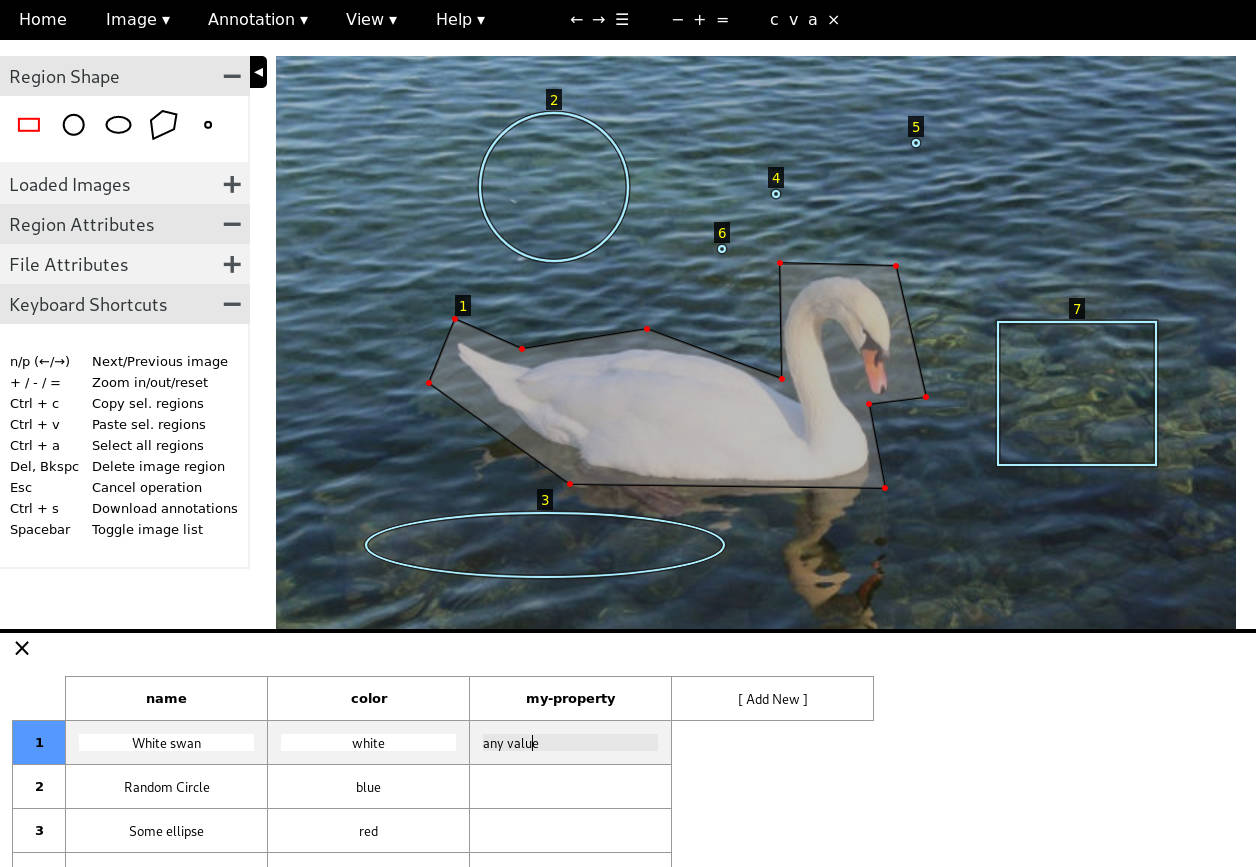
\includegraphics[width=\textwidth]{img/via.jpg}
%         \caption{VIA}
%     \end{subfigure}
%     \hfill
%     \begin{subfigure}[b]{0.42\textwidth}
%         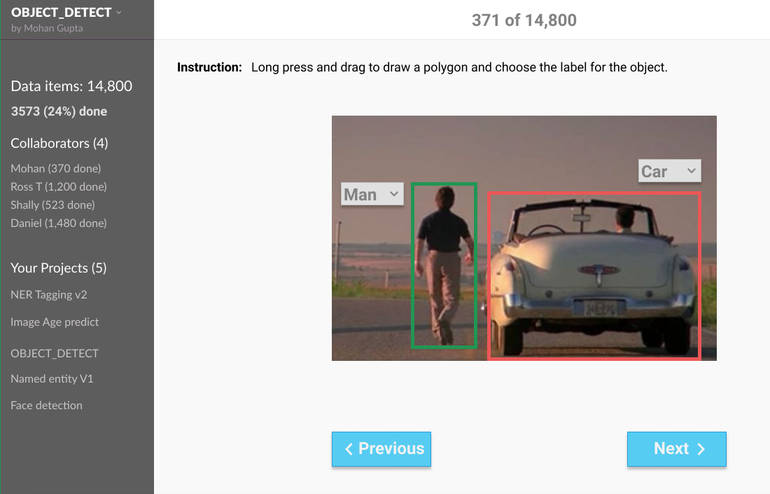
\includegraphics[width=\textwidth]{img/dataturks.jpg}
%         \caption{Dataturks}
%     \end{subfigure}
%     \hfill
%     \begin{subfigure}[b]{0.56\textwidth}
%         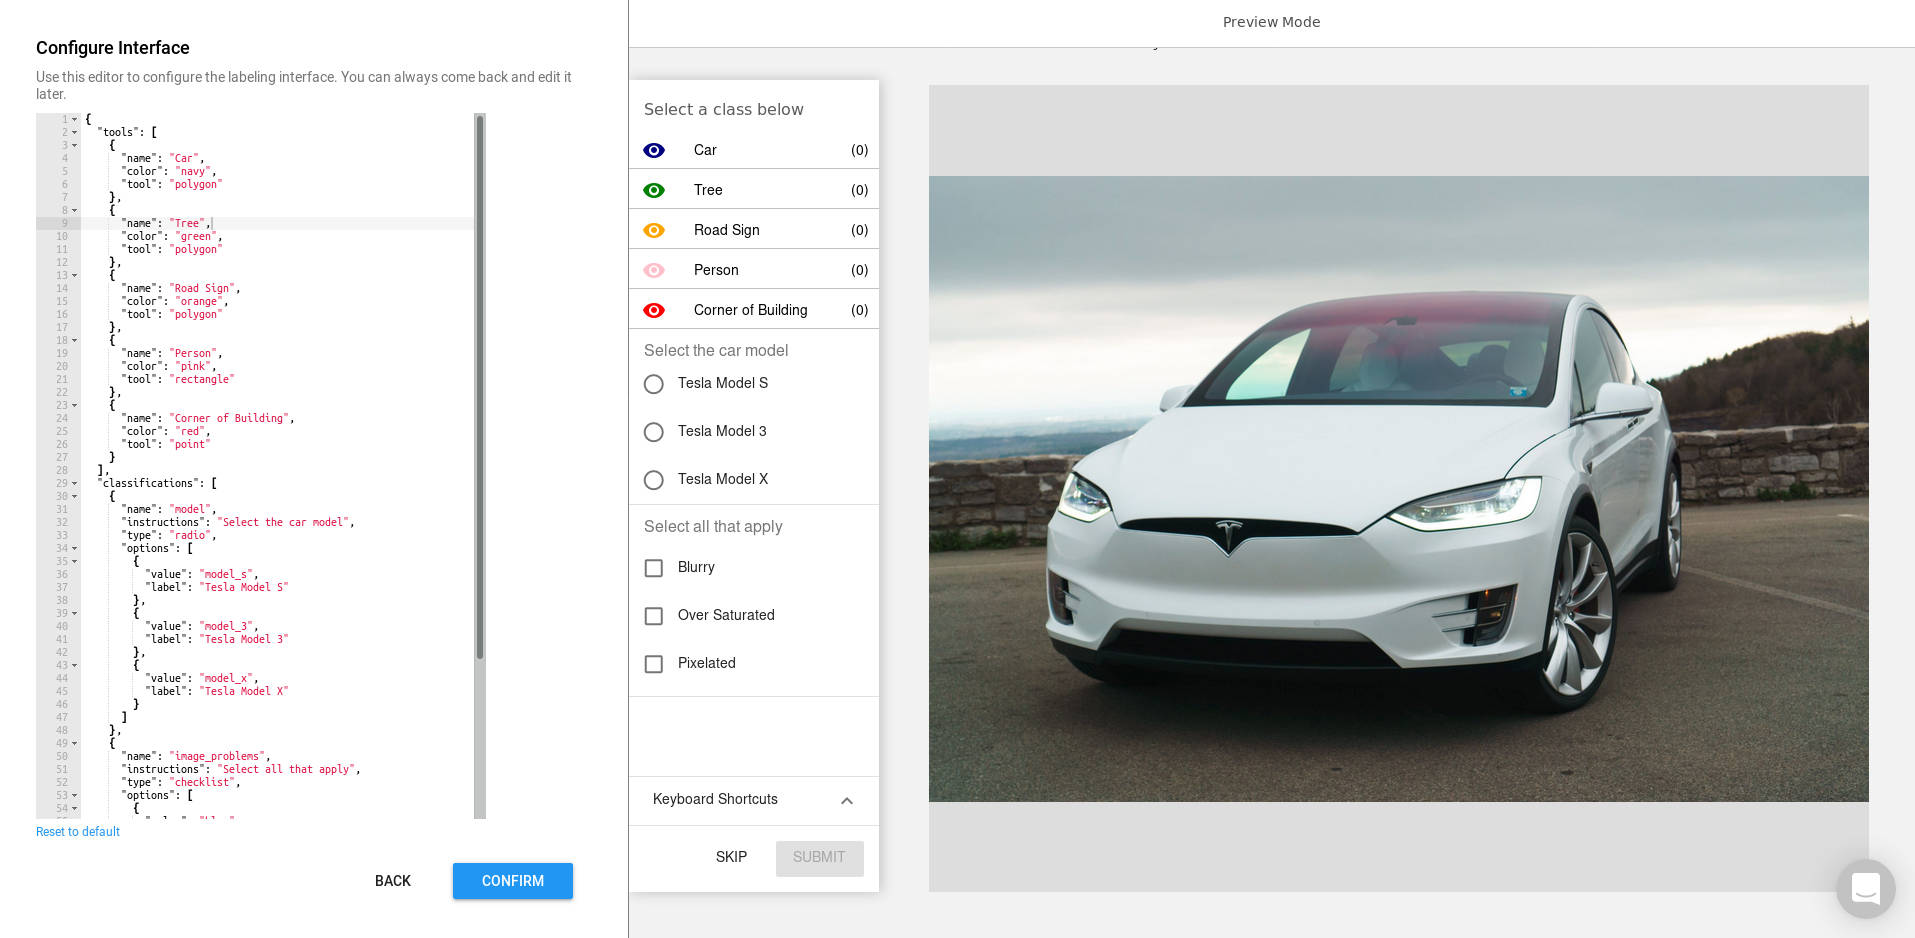
\includegraphics[width=\textwidth]{img/label-box-config.jpg}
%         \caption{Labelbox}
%     \end{subfigure}
%     \caption{Interfaces of main other Web annotation applications}\label{fig:interfaces}
% \end{figure*}

Many applications exist for image annotation (Table~\ref{tab:web-apps}).
One of the most popular is LabelMe~\cite{russell2008labelme}.
LabelMe provides an interface for drawing bounding boxes and polygons
around objects in an image,
and has been used extensively to create datasets for image segmentation.
Some more recent softwares share the same goals, with various particular features.
For example, Labelbox~\cite{labelbox} and
Dataturks~\cite{dataturks} provide tools for annotation tasks management,
particularly useful when crowdsourcing the annotations;
these softwares are proprietary.
The VGG Image Annotator (VIA~\cite{dutta2016via})
is an open source client application like ours,
with the particularity of providing annotation attributes,
editable in a spreadsheet format.

We release an open-source application~\cite{annotationappgithub},
purely client side, meaning that no data is uploaded to any server.
Images are loaded from files and annotated locally, in the browser.
The simplest tool, from a user perspective, should be immediately available
i.e.\ should not require any additional installation to be fully functional.
Our image annotation tool is thus a Web-based application,
easily configurable to fit users needs, as well as
embeddable in the Mechanical Turk platform to design crowdsourcing campaigns.

We first present the features of our application, then describe its architecture.
Finally, we explain how it can be used to start crowdsourcing experiments.

\section{Presentation of the application}

A screenshot of the application can be seen in Figure~\ref{fig:teaser}.
The image to be annotated occupies the central part of the screen;
a toolbar is located on top, object classes are available on the left
and images to be annotated on the right.


\textbf{Images}.
Multiple images can be loaded at the same time using the image icon
on the top-right corner of the application.
These images are not uploaded on the server,
and can either be loaded locally from the client's machine,
or from a distant server.
% * <matthieu.pizenberg@gmail.com> 2018-05-20T06:53:31.040Z:
% 
% > or from a distant server.
% Seulement quand c'est fait directement dans le champ images des "flags" au démarrage de l'appli, pas en cliquant sur le bouton
% 
% ^ <matthieu.pizenberg@gmail.com> 2018-05-20T09:57:23.955Z.


\textbf{Tools}.
Our application includes several tools to annotate images.
Icons for these tools are depicted in Figure~\ref{fig:icons}.
From left to right, the first available annotation is the point,
that can be useful to designate objects in the image.
It can also be used as a seed in region-growing image segmentation methods.
The second annotation we included is the bounding box,
which provides the localization of objects in the image,
and is used in object detection problems.
The information we acquire are the left, right, top and bottom coordinates
of the bounding box.
The third annotation we chose to implement is the stroke,
or scribble, which is a popular interaction in image segmentation.
It consists in a sequence of points, interpreted as a continuous line.
The outline, fourth type of annotation,
is a closed shape, typically drawn around objects.
It is comparable to a bounding box in essence,
but provides a more precise location of objects.
Finally, polygons can also be drawn (as in LabelMe, for instance),
by successively clicking new points as vertices.


All these tools are available both with a mouse or a touch interaction.
As a matter of fact, some tools are better suited to touch devices
(for example, outlines) than others (polygons).

\begin{figure}[ht]
\centering
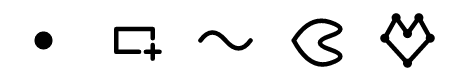
\includegraphics[width=0.8\columnwidth]{img/annotation-tools.png}
\caption{Annotation tools icons}%
\label{fig:icons}
\end{figure}


\textbf{Object classes}.
For most annotation tasks, we also need to differentiate objects in the images.
Typically each annotated area is attributed a class, or label.
The PASCAL VOC dataset~\cite{everingham2010pascal}, for example,
is composed of 20 classes, grouped by categories:
\begin{itemize}
\item \textit{Person}: person
\item \textit{Animal}: bird, cat, cow, dog, horse, sheep
\item \textit{Vehicle}: aeroplane, bicycle, boat, bus, car, motorbike, train
\item \textit{Indoor}: bottle, chair, dining table, potted plant, sofa, tv/monitor
\end{itemize}

In our application, classes are specified in a JSON configuration file.
A strict corresponding config for PASCAL VOC classes
is presented in Listing~\ref{lst:pascal}.

\lstinputlisting[language=json,caption={A configuration file to annotate the PASCAL dataset.},float,label={lst:pascal}]{code/config-pascal.json}

To attribute a class to an annotation,
a user should first select the class in the left sidebar,
then use a tool to create an annotation.
Selecting a class in the left sidebar also highlights the annotations
corresponding to this class.


\textbf{Configuration file}.
The five annotation tools are optionally made available by the configuration file.
In Listing~\ref{lst:pascal}, the last line of the depicted configuration file
contains an \texttt{annotations} field, listing the tools that should be available.
In this case, they all are.

In addition to the five fundamental annotation types,
each type can be derived in virtually any number of variations.
For example, interactive segmentation algorithms often require
\textit{foreground} and \textit{background} scribbles.
In our application, this would mean the user would need to draw two types of strokes.
This can be achieved using the configuration file,
as in Listing~\ref{lst:variations}.
Such configuration would result in two stroke icons in the toolbar,
of different colors, just as in Figure~\ref{fig:teaser}.

\lstinputlisting[language=json,caption={A configuration file to include two types of strokes.},float,label={lst:variations}]{code/config-variations.json}


\section{Technical choices}

The application is organized in two parts:

\begin{itemize}
\item A minimalist Nodejs server, located in the \verb|server/| directory.
	It is statically serving the content of \verb|server/dist/|
    with compression.
\item A complete Elm client application, located in the \verb|client/| directory.
    Elm~\cite{czaplicki2013asynchronous,czaplicki2017elm}
    isn't a JavaScript framework, it is a functional programming language,
	compiling to JavaScript to run in browsers.
	Its syntax is inherited from Haskell but far simpler.
	The compiled application is 150 KB gzipped,
    which is great for low bandwidth connections.
\end{itemize}


\subsection{The application architecture}

\begin{figure}[ht]
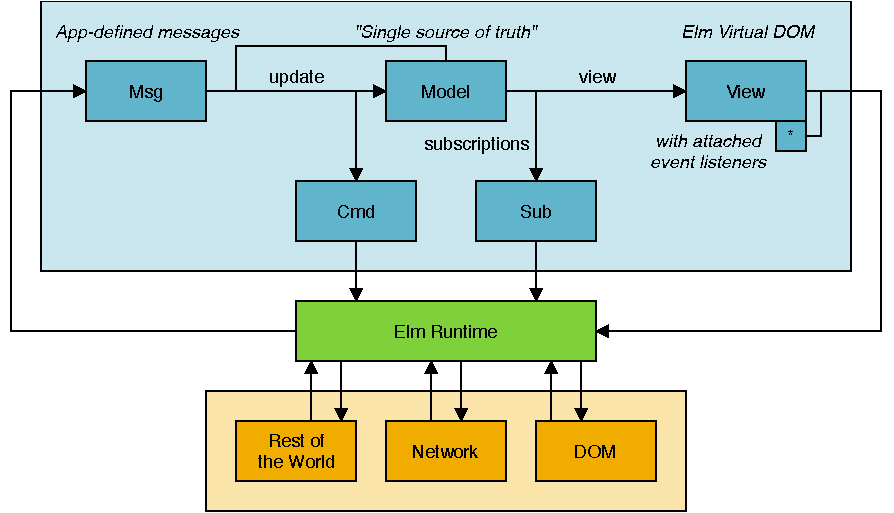
\includegraphics[width=\columnwidth]{img/tea-draw-io.pdf}
\caption{The application architecture.}%
\label{fig:tea}
\end{figure}

The application architecture enforces a unidirectional data transformation flow,
visualized in Figure~\ref{fig:tea}.
The central entity is the \verb|Model|.
It contains all and every information about our application state.
The visual aspect of our application is called the \verb|View|
(basically an HTML document) which is generated by the \verb|view| function,
from the \verb|Model|. Finally, all events generate messages, of type \verb|Msg|.
The \verb|update| function, updates the model by reacting to those messages, closing the loop.

All Elm functions are pure, meaning there is no side effect,
outputs of functions are entirely defined by inputs.
There cannot be global variables access,
real world events, network interaction etc.
Basically such a program would be running in a predestined way
from its start to its end,
preventing us from loading images and interacting with them.
This is why the application is attached to the Elm runtime,
provided by the language, transforming all real world events (``side effects'')
into our defined set of messages, of type \verb|Msg|.

The main challenge with pure functions is
to describe side effects without performing them.
Those are described in three locations:

\begin{enumerate}
\item View attributes as DOM event listeners for pointer events.
\item Commands (\verb|Cmd|) generated by the update function, like loading of images.
\item Subscriptions (\verb|Sub|) to outside world events like the window resizing.
\end{enumerate}

The Elm runtime takes those side effect descriptions,
perform them, and, whenever there is a result / an answer,
transforms it into one of our defined messages (\verb|Msg|)
and route it to our update function.


\subsection{The model states}

The \verb|state| is the main component of the \verb|Model|.
It contains the images and configuration loaded as well as the annotations performed.
Its type is defined as in Listing~\ref{lst:state}
and can be modeled as a finite state machine, visualized in Figure~\ref{fig:states}.

\lstinputlisting[language=haskell,caption={State type definition.},label={lst:state},float]{code/State.txt}

\begin{figure}[ht]
\centering
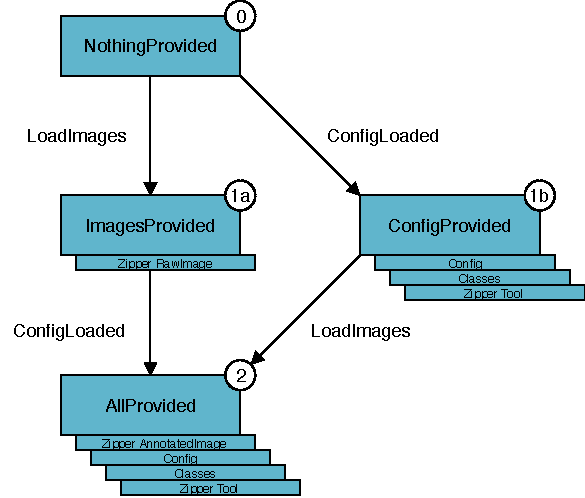
\includegraphics[width=\columnwidth]{img/states-draw-io.pdf}
\caption{The application states.}%
\label{fig:states}
\end{figure}

The application available online starts in state 0 (\verb|NothingProvided|)
and enables you to reach state 2 (\verb|AllProvided|)
with buttons to load images and configuration.
Two messages called \verb|LoadImages| and \verb|ConfigLoaded| produce
transitions in the state machine.


\subsection{The messages}

All modifications of the model are understood
by looking at the \verb|Msg| type definition (Listing~\ref{lst:msg}).
The \verb|update| function then performs the modifications described by those messages.

\lstinputlisting[language=haskell,caption={Msg type definition.},label={lst:msg},float]{code/Msg.txt}

\begin{itemize}
\item The \verb|WindowResizes| message is triggered when the application is resized.
	In the update function, it takes the new size and recomputes some view parameters.
\item A \verb|PointerMsg| message is triggered by pointer events (mouse, touch, etc.).
	In the update function, this is the message activating
	all the annotations logic code of our application.
\item The messages \verb|SelectImage|, \verb|SelectTool| and \verb|SelectClass|
	are generated when clicking on images, tools and classes.
\item Files are handled by five messages:
	\begin{itemize}
	\item When selecting images in the file explorer to load,
		a \verb|LoadImages| message is generated with a list of the images files
		and their names as identifiers.
		For each image correctly loaded an \verb|ImageLoaded| message is generated,
		providing a local url, corresponding to the image in memory.
    \item The messages \verb|LoadConfig| and \verb|ConfigLoaded| behave similarly.
    \item The \verb|Export| message causes the application to serialize into Json
		all the annotations, and asks the user to save the generated file.
		It is triggered by clicking on the export button of the top action bar.
	\end{itemize}
\item Whenever an event should change the zooming level of the drawing area,
	a \verb|ZoomMsg| message is  generated.
\item Finally, the \verb|RemoveLatestAnnotation| message is also explicit.
\end{itemize}


\subsection{The view}

The view of this application is based on four components,
each implemented in its own module, with potentially different versions
depending on the current state of the application.
\begin{itemize}
\item The top action bar (\verb|src/View/ActionBar.elm|).
\item The center annotations viewer area\\(\verb|src/View/AnnotationsArea.elm|).
\item The right images sidebar\\(\verb|src/View/DatasetSideBar.elm|).
\item The left classes sidebar\\(\verb|src/View/ClassesSideBar.elm|).
\end{itemize}


% \subsection{Startup and interactions with JavaScript}

% Compiling the Elm application code produces a JavaScript file \verb|Main.js|.
% This file has to be embeded in an html document.
% Then the application is started with parameters called "flags"
% as demonstrated in Listing~\ref{lst:start}.

% \lstinputlisting[language=javascript,caption={JavaScript code to embed the Elm application.},label={lst:start},float]{code/start.js}


\subsection{Library and application duality}

In order to offer a turnkey solution to image annotations,
we created a configurable application solving most needs.
But we also thought of cases where advanced modifications are required.
Consequently, the foundation of this application has been extracted
in the independent package elm-image-annotation~\cite{annotationpackage}.
It is designed as an API to create, modify and visualize geometric shapes,
useful in the context of image annotation.

Modules for manipulation and serialization (in JSON) of annotations are
under the \verb|Annotation.Geometry| namespace.
It already contains one module for each tool presented earlier.
If you want to introduce a new tool, this is where you can create a new module.

This package also contains the following important modules,
under the \verb|Annotation| namespace:
\begin{itemize}
	\item \verb|Annotation.Style|:
		defines types describing appearance of points, lines and fillings of annotations.
	\item \verb|Annotation.Svg|:
		exposes functions rendering Svg elements for each annotation kind.
	\item \verb|Annotation.Viewer|:
		manages the central visualization are,
		supporting zooming and translations, relative to an image frame.
\end{itemize}
If you are interested in creating another rendering target than SVG,
like canvas, WebGL, \ldots, it would require alternative modules
to \verb|Annotation.Svg| and \verb|Annotation.Viewer|.
The rest of the code can stay unchanged.

\section{Crowdsourcing annotations}

Image annotation interfaces are often used in the context
of large datasets of images to annotate.
As such, tasks management for crowdsourcing campaigns is an important feature. 
Labelbox and Dataturks are all-in-one services providing
tasks management directly in their applications.
Just like LabelMe, we choose instead to provide a configuration,
ready to use with Amazon Mechanical Turk (Mturk).

Mturk comes in two sides. A ``requester'' is defining a set of tasks
while a ``worker'' is performing them.
Workers are payed by requesters through Mturk service.
The concept of a ``HIT'' (Human Intelligence Task) characterizes the task unit.
In our case, one HIT means one image to be annotated.
We describe in details how to setup a campaign with our template
in the application documentation.
\section{Conclusion}

In this paper we have introduced our web-based image annotation application.
More information is available on the documentation pages~\cite{annotationappdoc}.
The application is still actively developed, we welcome all feedback and contributions.

\begin{acks}

We would like to thank:

\begin{itemize}
	\item @tforgione and @GarciaDelMolino for your wise feedbacks.
	\item @dncg for your Windows tests.
	\item The online Elm community for their help along the road:
		@evancz for the delightful Elm language,
		@ianmackenzie for your fantastic geometry library,
		@mdgriffith for your very refreshing layout library,
		@luke for the amazing tool Ellie,
		@norpan, @jessta, @loganmac, @antew, for your invaluable help on slack.
\end{itemize}

\end{acks}


\bibliographystyle{ACM-Reference-Format}
\bibliography{main}

\end{document}
